\beginsong{In Junkers Kneipe}[wuw={Julia Schäfer, 1936}, bo={212}]

\markboth{\songtitle}{\songtitle}

\beginverse
\endverse

\centering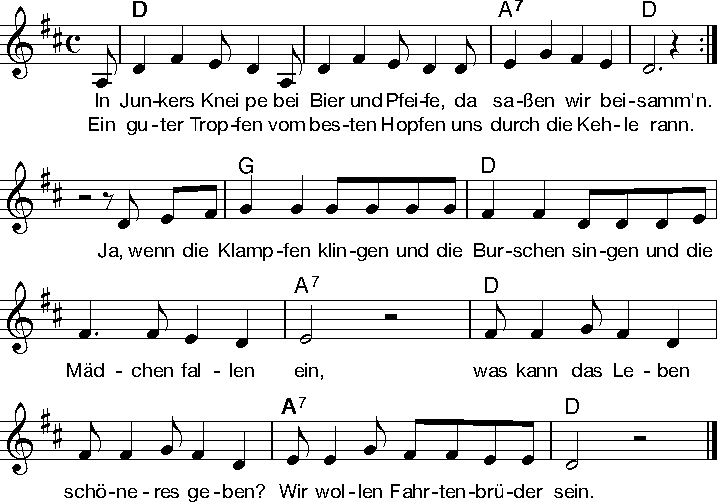
\includegraphics[width=1\textwidth]{Noten/Lied054.pdf}	

\beginverse
Die \[D]alten Zeiten vorüber gleiten und \[A7]draußen tobt die \[D]Nacht.
Und \[D]immer wieder singen wir die Lieder, die \[A7]uns so froh ge\[D]macht.
\endverse

\beginchorus
Ja, wenn die \[G]Klampfen klingen und die \[D]Burschen singen
und die \[A7]Mädchen fallen ein:
\[D]was kann das Leben schöneres geben?
\[A7]Wir wollen glücklich \[D]sein!
\endchorus

\beginverse
\endverse 

\beginverse
Es ^ist so spät schon, der Wirt, der schläft schon, das ^Bier wird langsam ^schal.
Doch ^eh' wir gehen, zum Schlaf uns legen, da ^singen wir noch^mal:
\endverse

\renewcommand{\everychorus}{\textnote{\bf Refrain (wdh.)}}

\beginchorus
\endchorus

\endsong

\beginscripture{}
''In Junkers Kneipe'' war in der Zeit des Nationalsozialismus vor allem in den Widerstandsgruppen bekannt. Die heutige Version ist von einer Gruppe Mülheimer Edelweißpiraten überliefert. Andere Versionen sprechen den Widerstand gegen den Nationalsozialismus offener an. So heißt es in einer Überlieferung ''Wo die Fahrtenmesser blitzen und die Hitlerjungen flitzen und wir Edelweißpiraten schlagen ein...''
\endscripture

\begin{intersong}

\ifthenelse{\boolean{pics}}{
\vspace{30pt}
\centering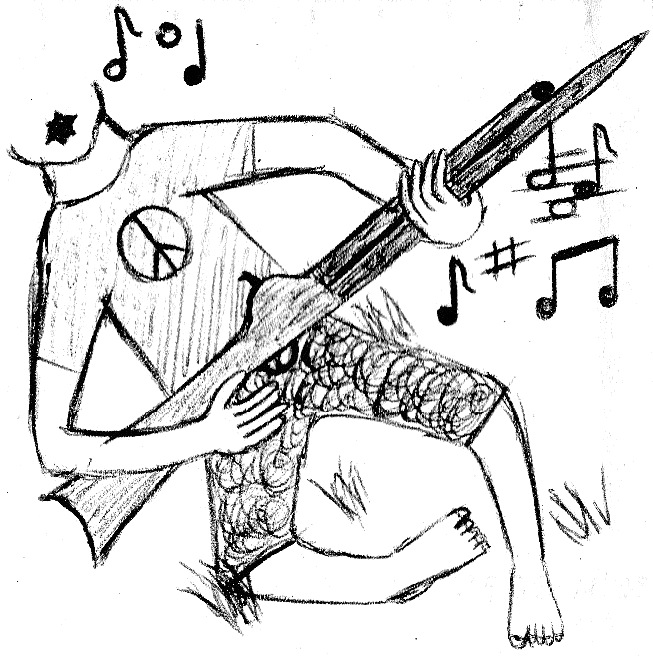
\includegraphics[width=0.8\textwidth]{Bilder/injunkers_mikesch.jpg}
}{}

\end{intersong}